\chapter{Background Research}
\label{chapter2}

% \section{Problem Overview}
% \lipsum[1-1] \cite{parikh1980adaptive}

This section expands on the background the project is covering which is virtual reality. This research was conducted to understand the current state of virtual reality and what bleeding edge technology platforms can offer to be used in the development in this project.

\section{Virtual Reality}
	Virtual Reality is a technology that has been around since the early 19th century, although in a primitive form through the use of stereoscopic photos \cite{stereoscopy}. Stereoscopic photos work by using two photos that are taken of the same place but are slightly offset from each other, as can be seen in \ref{fig:stereoscope1}. This creates an illusion of depth for the person viewing the images, when viewed through a stereoscope. A stereoscope is a viewing device that only allows one eye to see one of the two images, so each eye sees a similar, yet different image, and this gives the illusion of depth. Stereoscopic vision is the same technology used in current Virtual Reality headsets although now the images are moving.

\begin{figure}[h]
	
\includegraphics[width=10cm]{stereoscope}
	\centering
	\caption{Example of a stereoscopic image. \cite{leedsstereoscopic}}
	\label{fig:stereoscope1}
\end{figure}

There are a few more requirements for virtual reality platforms to consider in order to achieve an immersive experience and reduce motion sickness. A core fundamental feature of virtual reality is the ability to track head movements of the player in order for the game camera to adjust itself accordingly. IMU (inertial measurement unit) is a self-contained system in the headgear which measures linear and angular motion using multiple gyroscopes and accelerometers \cite{imu}. The device's IMU must be optimised and precise to provide accurate movement data as fast as possible since latency is another key factor.
\newline
\par
Latency as in most occasions is important to be reduced especially in virtual reality. Latency is the amount of time for a player action to be sent and registered to the game then for the game logic to compute this and display the consequence on the player's display. In the case of virtual reality, this would be the time for head movement to be registered and  the game to change the camera perspective to display in the virtual headgear. High latency would mean that the player will be seeing a delayed response of their actions which increases motion sickness as the brain is not seeing the expected response in a timely manner. This breaks the immersion and greatly increases chances of nausea and motion sickness.
\newline
\par
Another cause of possible motion sickness is the refresh rate of the headgear's displays. The refresh rate of a display is the amount of times a display updates it's image on the screen in a second. This also means that the refresh rate will determine how frames per second generated by a game will be displayed on the screen. A higher refresh rate display will allow games that can perform better by generating more frames per second seem smoother to the player's eyes. A low refresh rate would also introduce latency since the player's action cannot be displayed as quickly on the screen.
\newline
\par
Another key component of virtual reality that needs to be considered is the resolution of the display's screen. The resolution of a display is the amount of pixels that can be shown on the display so a higher resolution would mean a finer, more sharp image can be shown. This is important in virtual reality since the display is only millimetres away from the user's eyes so it would be easier for the user to distinguish individual pixels if the resolution is low.
\newline
\par
Virtual reality platforms have been released aiming to provide an immersive experience to consumers. There are many varieties currently available and they can be simply separated in to the two categories: mobile and desktop. Mobile experiences such as the Google Cardboard and Samsung's Gear VR target the audience which already own a compatible mobile device thus eliminating the cost of hardware found in higher end platforms. Through the use of the phone's built in gyroscope and accelerometer, crude head tracking can be achieved to emulate a virtual world.
\newline
\par
High end virtual reality platforms target enthusiasts and early adopters of cutting edge technology due to its premium price and high computer hardware requirements in order to run it. Currently there are two virtual reality headsets that are seen as the devices that give highest immersion and these are Facebook's Oculus Rift and HTC's Vive. These will be discussed later in this chapter.

\subsection{Mobile VR}
On the market right now there are two main mobile virtual reality hardware. There is the Samsung Gear VR and the Google Cardboard.

\subsubsection{Google Cardboard}
The Google Cardboard is the cheapest Virtual Reality headset out on the market right now, but it does come with the least features out of them. The cardboard viewer is a stereoscope made out of cardboard. It contains two 40mm focal lenses that are designed to give a distortion when looking through them, which is counter-acted by the distortion from the application\cite{cardboarddev}.
\newline
\par
To use the Google cardboard you would need to install the cardboard application on your compatible phone and then place your phone inside of the Google Cardboard. Once the phone is inside the Cardboard it uses the phone's IMU to track head movement. This does have limitations however as the Google Cardboard does not track displacement if the user was to walk in any direction.
\newline
\par
The Google Cardboard still uses the technology of stereoscopic images, as can be seen in \ref{fig:cardboard1}. Although it now does it with moving images, which creates a more immersive experience. \\

\begin{figure}[h]
	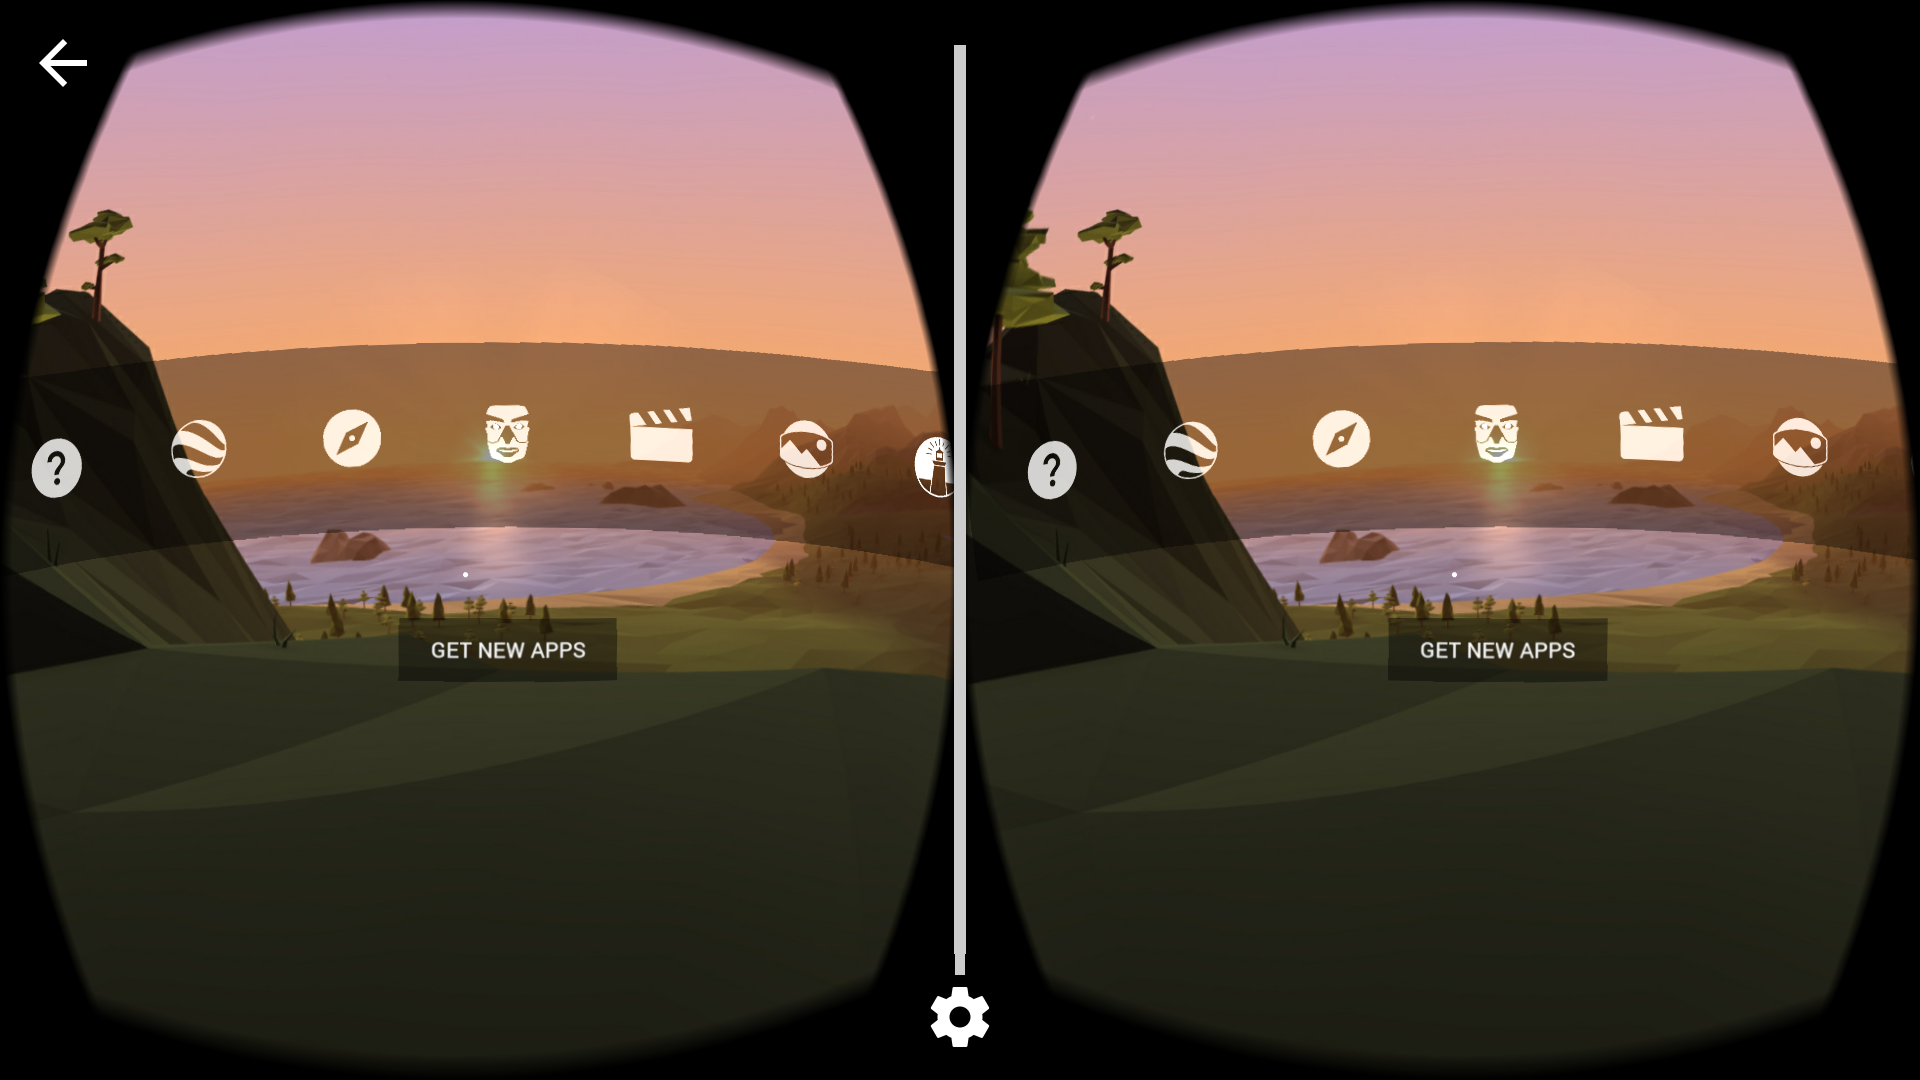
\includegraphics[width=\textwidth]{cardboardscreen}
	\centering
	\caption{Image showing the Cardboard demo application}
	\label{fig:cardboard1}
\end{figure}

The Google Cardboard was not chosen to the virtual reality device for this project as there are many drawbacks to it, and as such it does fully demonstrate all the features present in modern technology for virtual reality. The drawbacks to the Google Cardboard are:

\begin{itemize}
	\item No displacement tracking, making it less immersive than the other options
	\item Only one input method, a button on the cardboard which acts as a screen press.
\end{itemize}

\subsubsection{Samsung Gear VR}
The other mobile Virtual Reality headset on the market is the Samsung Gear VR. The Samsung Gear VR is slightly more expensive than the Google Cardboard, and as expected with the price increase, it comes with more features compared to the Google Cardboard.
\newline
\par
The Samsung Gear VR uses the same technology as the Google Cardboard in the sense that it uses stereoscopic imaging to create the illusion of depth. This is done in the same way for both VR devices, by inserting a compatible phone into the phone holder in the headset, and then showing the stereoscopic images on the phone screen. As seen in \ref{fig:gearscreen} the Samsung gear VR uses the same stereoscopic technology as the Cardboard uses, as seen in \ref{fig:cardboard1}.
\newline
\par
The Samsung Gear VR also uses an inertial measurement unit to detect head movement, similar to the Google Cardboard. The Samsung Gear VR uses an inertial measurement unit contained in the headset, rather than using the attached phone's inertial measurement unit. The inertial measurement unit contained in the headset is more accurate, has lower latency, and is better calibrated than standard phone inertial measurement units, as it uses the same I.M.U. as the Oculus Rift. This I.M.U. is more accurate as it has a higher sample rate than internal phone I.M.U.s and therefore gives it more values to use, so that it can more accurately detect erroneous values.

\begin{figure}[h]
	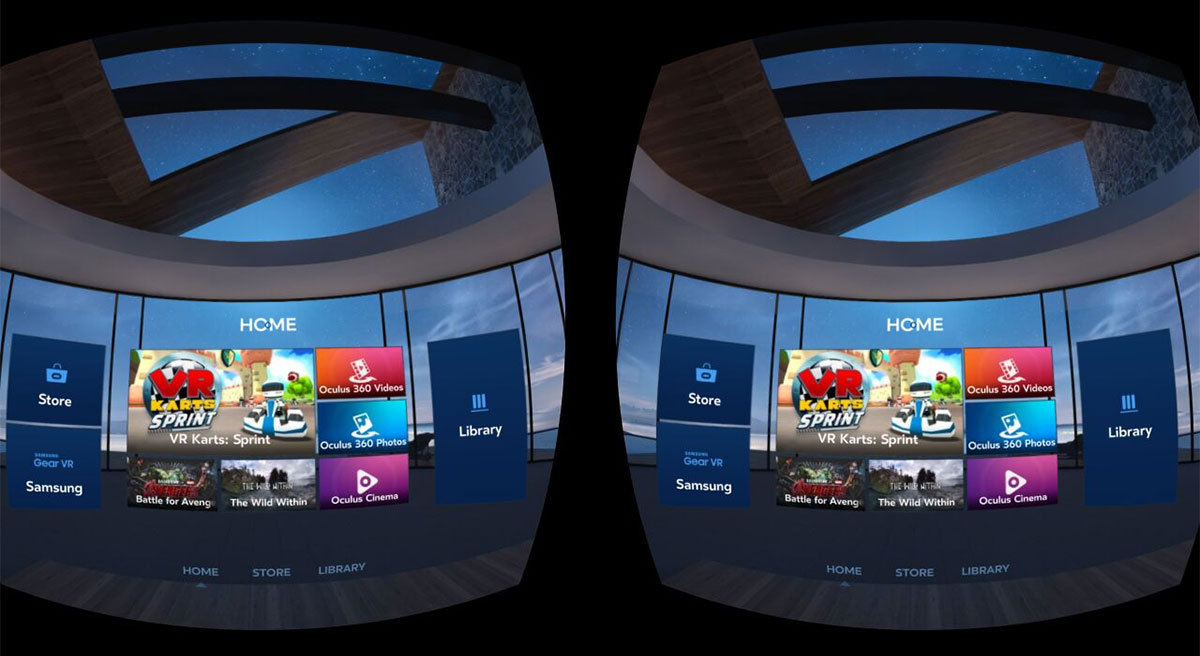
\includegraphics[width=\textwidth]{gearscreen}
	\centering
	\caption{Image showing the Samsung Gear VR menu \cite{gearmenu}}
	\label{fig:gearscreen}
\end{figure}

The Samsung Gear VR has a few extra features compared to the Google Cardboard, for example when a phone is placed inside the Galaxy Gear VR it needs to be connected by a micro-usb connection, which allows the headset to have more input methods to the phone, as well as giving access to the headset's I.M.U. The extra input methods that the Gear VR has access to are:\\

\begin{itemize}
	\item A home button, which works the same as the home button on Android phones.
	\item A back button, which works the same as the back button on Android phones.
	\item A touch pad, which works by swiping to move across menus, and tapping clicks the highlighted item in a menu.
\end{itemize}

\begin{figure}[h]
	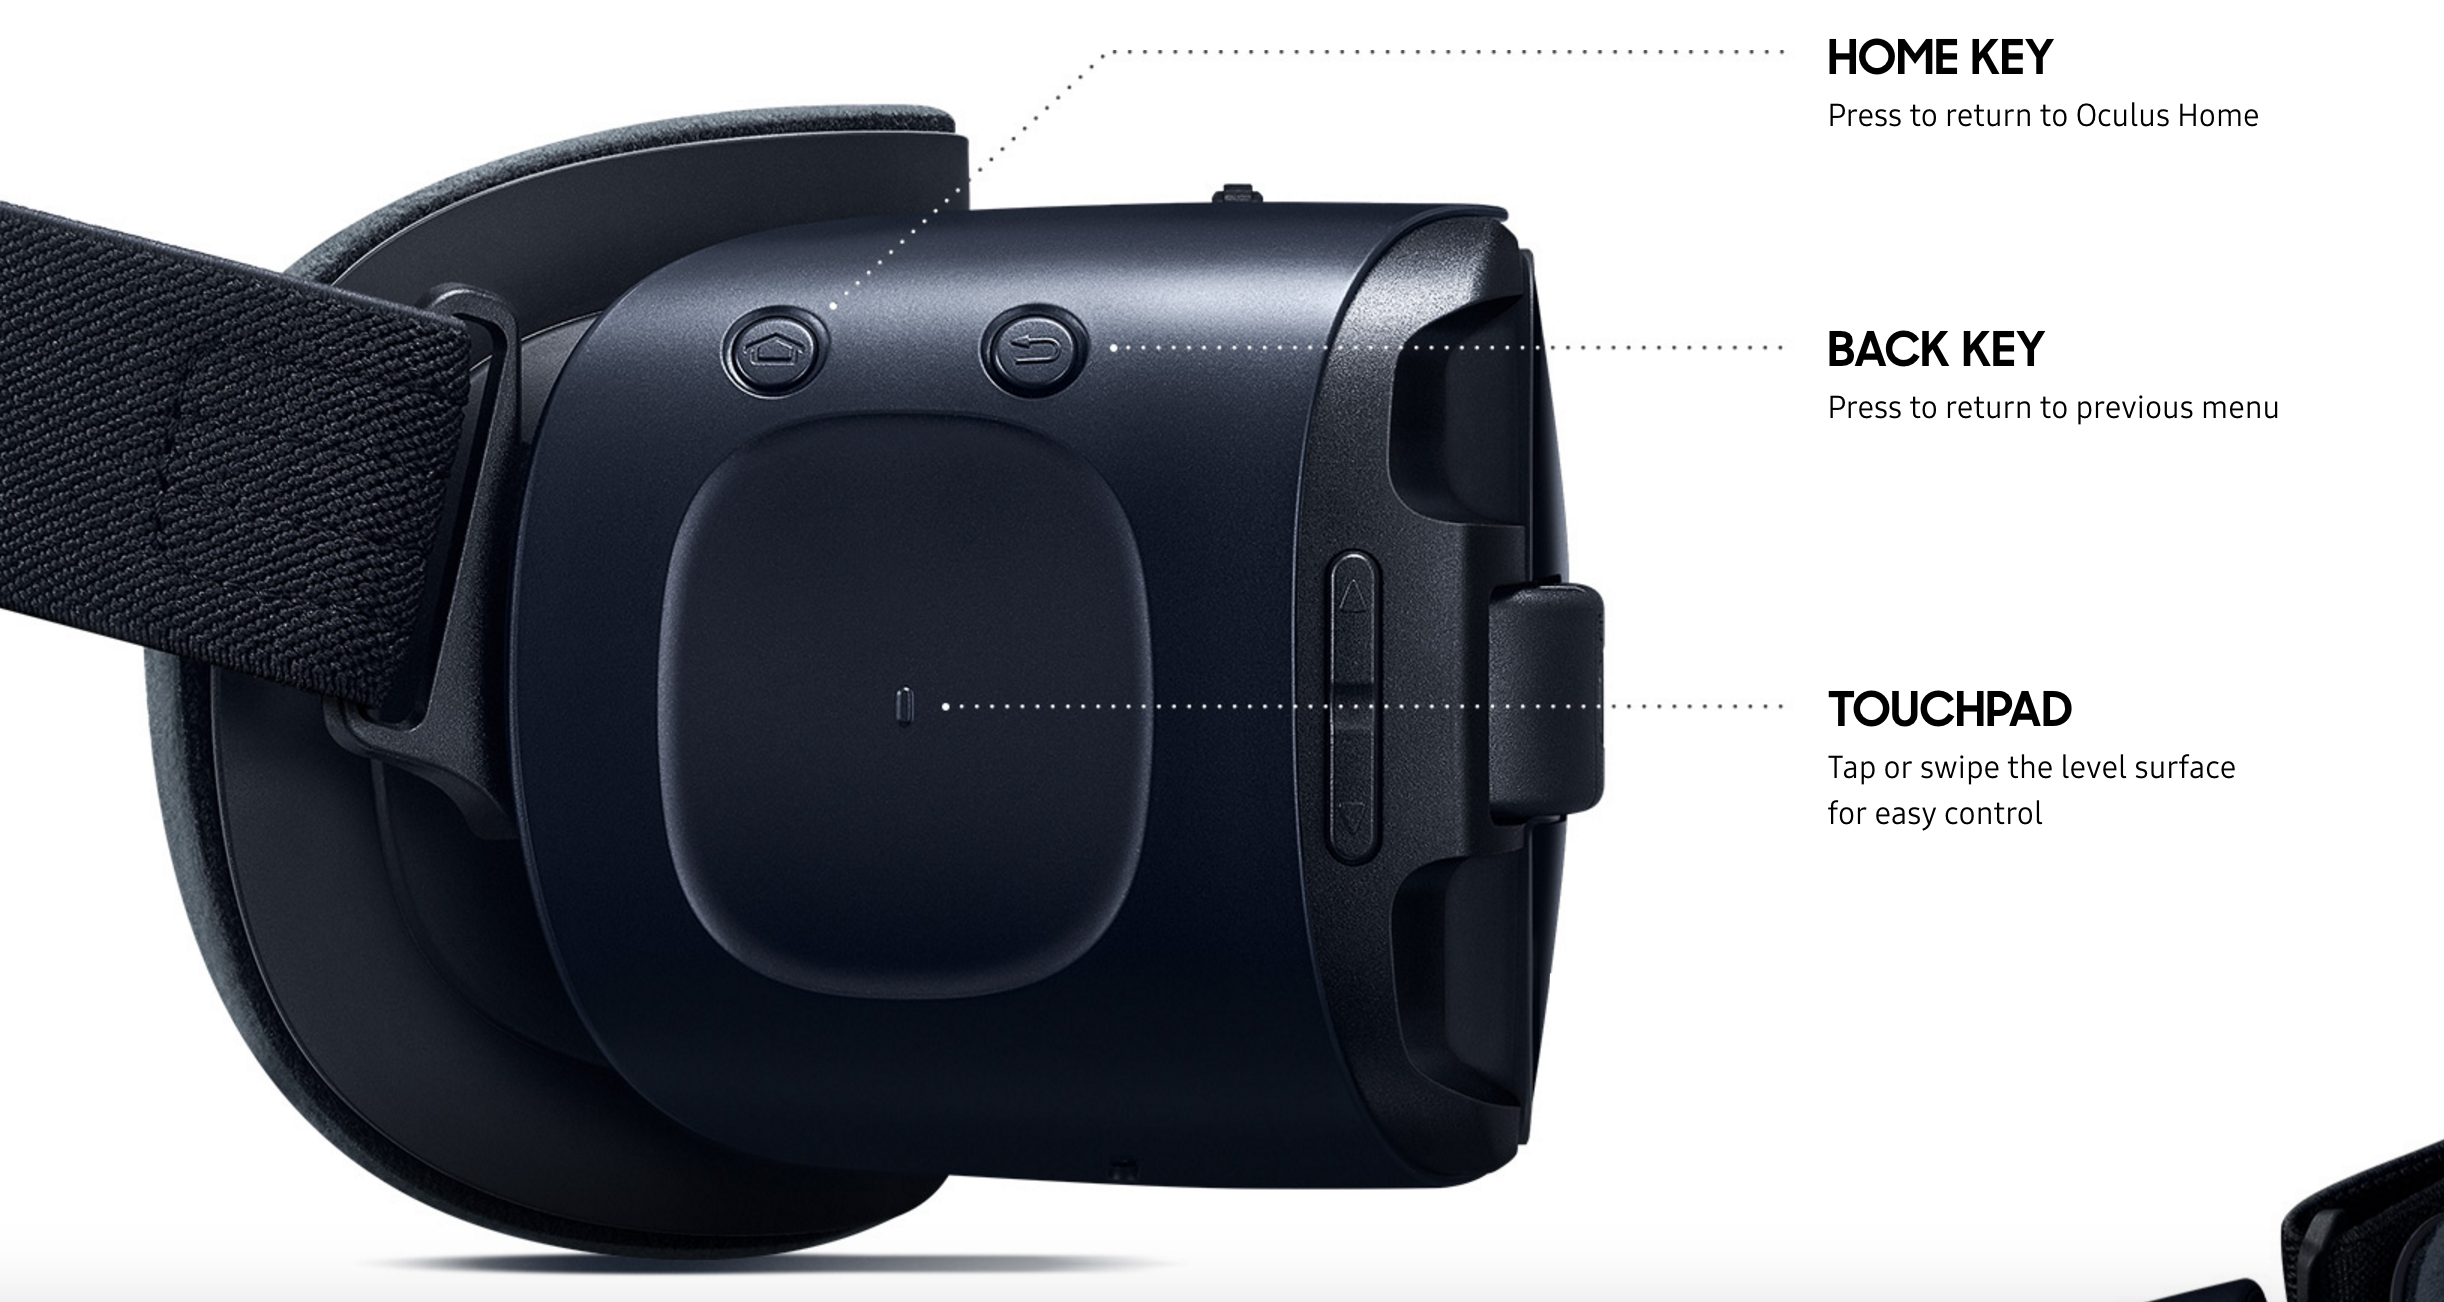
\includegraphics[width=13cm]{gearcontrols}
	\centering
	\caption{Image showing the hardware controls on the Samsung Gear VR \cite{gearbuttons}}
	\label{fig:gearcontrols}
\end{figure}

The Samsung Gear VR will not be used for this project as again it has several drawbacks, which are:

\begin{itemize}
	\item It only tracks rotational movement, not displacement, which makes it less immersive than the other options
	\item The Samsung Gear VR has very primitive control, which are only the buttons and touchpad on the side of the headset
\end{itemize}		

\subsection{Oculus Rift}
The Oculus Rift was the first of the two to be released and is inferior in terms of the level of immersion that can be achieved, as currently Oculus only supports interfacing with the virtual world through a third party traditional controller that simply uses buttons and joysticks. The Oculus Rift tracks by using the single camera to pick up infra-red light that is emitted by points on the headset. These can be used to track the headset as they blink in a specific pattern, which the sensor knows, and it then uses that to determine the position the headset is in.

\subsection{HTC Vive}
The HTC Vive works using two base stations. These emit lasers in an alternating pattern, between vertical and horizontal. If these lasers hit a sensor on the headset or controllers, they emit a pulse. By tracking the timings of the laser sweeps and the emitted pulses, the tracking system can use trigonometry to find the position of the location of every sensor on the devices \cite{vivetechnology}. The HTC Vive has two settings, either a sitting or a standing mode. In the sitting mode, it works similar to the Oculus Rift, in that a gamepad is used to control the game, where as in the standing mode, it uses it's own controllers. The motion controllers which are tracked by the base stations provide a more immersive experience as it gives the player a more natural interaction with the virtual world. For example it allows the player to interact with objects in the game by using these controllers to pick things up by the player moving their hands to where the object is in game.
\clearpage

\subsection{Summary of VR Solutions}

\begin{table}[ht]
\centering
\begin{tabular}{|l|l|l|}
\hline
 & \textbf{Google Cardboard} & \textbf{Gear VR} \\ \hline
\textbf{Display} & Varies & OLED \\ \hline
\textbf{Resolution} & Varies & 2560 x 1440 \\ \hline
\textbf{Refresh Rate} & 60Hz & 60Hz \\ \hline
\textbf{Field of View} & Varies & 90-96 degrees\cite{fov} \\ \hline
\textbf{Tracking Area} & Static & Static \\ \hline
\textbf{Controller} & One button & Buttons and touch pad \\ \hline
\textbf{Sensors} & Accelerometer, gyroscope & Accelerometer, gyroscope, phone camera \\ \hline
\textbf{Requirements} & \begin{tabular}[c]{@{}l@{}}\cite{cardboardreq}Android phone:\\ versions 4.1 or higher\\ \\ iOS phone:\\ versions 8.0 or higher\end{tabular} & \begin{tabular}[c]{@{}l@{}}Gear VR compatible phone:\\ S6, Note 5, S7\end{tabular} \\ \hline
\end{tabular}
\caption{Comparisons table of mobile VR}
\label{mobiletable}
\end{table}

\begin{table}[h]
\centering
\begin{tabular}{|l|l|l|}
\hline
 & \textbf{Oculus Rift} & \textbf{HTC Vive} \\ \hline
\textbf{Display} & OLED & OLED \\ \hline
\textbf{Resolution} & 2160 x 1200 & 2160 x 1200 \\ \hline
\textbf{Refresh Rate} & 90Hz & 90Hz \\ \hline
\textbf{Field of View} & 110 degrees & 110 degrees \\ \hline
\textbf{Tracking Area} & 5 x 11 feet & 15 x 15 feet \\ \hline
\textbf{Controller} & Xbox One Controller & Vive controller, any PC compatible gamepad \\ \hline
\textbf{Sensors} & \begin{tabular}[c]{@{}l@{}}Accelerometer, gyroscope, magnetometer,\\ Constellation tracking camera.\end{tabular} & \begin{tabular}[c]{@{}l@{}}Accelerometer, gyroscope,\\ Lighthouse laser tracking system,\\ front-facing camera\end{tabular} \\ \hline
\textbf{Requirements} & \begin{tabular}[c]{@{}l@{}}NVIDIA GeForce GTX 960 / \\ AMD Radeon RX 470 or greater\\ \\ Intel Core i3-6100 / AMD FX4350 or greater\\ \\ 8GB+ RAM\\ \\ Compatible HDMI 1.3 video output\\ \\ 2x USB 3.0 ports\\ \\ Windows 7 SP1 or newer\end{tabular} & \begin{tabular}[c]{@{}l@{}}NVIDIA GeForce GTX 970 /\\ AMD Radeon RX 480 equivalent or greater\\ \\ Intel Core i5-4590 equivalent or greater\\ \\ 4GB+ of RAM\\ \\ Compatible HDMI 1.3 video output\\ \\ 1x USB 2.0 port\\ \\ Windows 7 SP1 or greater\end{tabular} \\ \hline
\end{tabular}
\caption{Comparisons table of desktop VR \cite{oculusvive}}
\label{desktoptable}
\end{table}

HTC Vive virtual reality hardware was chosen since overall it is the best amongst all the current VR solutions. The display hardware compared to the Oculus is the same, but the Vive offers room-scale experiences where the player can move around world. Also, motion controllers can be used to interact with the virtual world. These gives more immersion and the ability to develop experiences using these features.

% \section{Gaming}
% \lipsum[1-1] \cite{parikh1980adaptive}
\clearpage
\section{Development Environments}
To develop on the HTC Vive there are two options which are currently supported and these are the Unity engine and the Unreal 4 engine\cite{vivedev}. These game engines has native support for SteamVR which is the platform developed by Valve that powers the Vive. Both are free to be installed and just requires a simple registration to their respective websites.

\subsection{Unity}
Unity is a cross-platform game engine by Unity technologies and was initially released on June 2005\cite{unitywiki}. It was first announced only for OS X, but since then 20 more platforms have been added support \cite{unityhistory}. The game engine has support for development of both 2D and 3D games which is why Unity is popularly used in mobile games such as Temple Run. The cross-platform integration means that games can be quickly and easily ported onto other platforms such as Android, iOS and Windows. Unity currently supports the C\# programming language as well as Javascript for the development of games.\cite{unity3d}. Unity is a free to download and develop in, but games built using this engine will have the Unity watermark if the Pro version is not used which is a paid license.

\subsection{Unreal Engine}
Unreal Engine is the other game engine that supports development for the HTC Vive. This game engine is developed by Epic Games and was initially released on July 1998 \cite{unrealwiki}. It was primarily developed for first-person shooter games but then has found success in various other genres such as stealth and role-playing games. The first native scripting language used for game code and gameplay events in Unreal was called UnrealScript. This first appeared in 1998 and was used up until 2014 when Unreal Engine 4 was announced. Unreal Engine uses C++ on its current version and with this it means it is more portable and can be used by many developers. Like Unity, Unreal Engine is free for game development and only requires a payment of 5\% royalty on games and applications that are released\cite{whatisunreal}. This will not be a problem since the project will only produce a tech demo for non-commercial uses.
\newline
\par
With the current version of Unreal, Unreal 4, development for previous generation consoles are no longer supported. UE4 games can be released on PC, Mac, iOS, Android, Xbox One and Playstation 4\cite{unreal4nextgen}. This means that the engine can fully take advantage of bleeding edge technology and higher end graphics without having to worry about older technology. An example of the improvement in graphics, UE4 can handle up to a million particles in a scene at one time whereas UE3 can only handle roughly a hundred.

\subsection{Unreal Engine: Choice for development}
Unity supports the C\# programming language for development whereas Unreal Engine uses C++ as its language of choice. Another aspect where it differs is Unity is mainly used to develop games for mobile devices such as 2D platformer games. Unreal Engine is mainly used for desktop, AAA games which makes it more suitable for virtual reality with games running on Unreal generally looking better.
\newline
\par
Unreal Engine includes many features built in such as particle effects simulation, terrain, lighting and shading \cite{unrealfeatures}. With SteamVR being natively supported, simple virtual reality features such as gesture recognition and teleportation movement mechanic can be easily implemented in to a game.
\newline
\par
For this project Unreal Engine will be used as the development environment. This is because the group is more comfortable with using C++ so development will be quicker with Unreal rather than trying to use a language with little familiarity. Syntax, grammar and structure of C++ will not be needed to be learnt and only special functions and members will be needed to be learnt and this can be easily done with the Unreal documentation. Along with Unreal's native VR support for headsets and motion controllers specifically for the Vive meant that learning to develop for the Vive will be easier.
\newline
\par
The Unreal Engine offers many features for people with little to no programming experience, these will not be used however, as they do not demonstrate any Computer Science expertise, one of the many features that will not be used is the drag and drop interface that is packaged in Unreal Engine to develop simple software quickly, along with the basic templates for various types of games. These are templates for popular genres, for example First Person Shooter and Sidescroller. For this project the group will implement their own features and back-end for the genre that is picked, in order to demonstrate their ability to code for the HTC Vive. A select list of the features that Unreal Engine implements already are as follows:

\subsubsection{Unreal Engine 4 Features}
\begin{itemize}

	\item Particle Effects Simulation (Visual Effects)
	\item Procedural Foliage
	\item Landscaping/Terrain
	\item Lighting

	\begin{itemize}
		\item Directional
		\item Point
		\item Spot
		\item Sky
		\item Shadow Casting
	\end{itemize}

	\item Shading
	\item Post Process Effects

	\begin{itemize}
		\item Bloom
		\item Ambient Occlusion
		\item Colour Grading
		\item Depth of Field
		\item Lens Flares
	\end{itemize}

	\item Material Effects
	\item Fog Effects
	\item View Distance Culling
	\item Distance Dependent Level of Detail Models
	\item Physics Simulation
	\item Level Streaming (Ability load and unload map files into memory and toggle their visibility)
	\item Basic Templates

	\begin{itemize}
		\item First-Person
		\item Third Person
		\item Side Scroller
		\item Vehicle
	\end{itemize}

	\item Artificial Intelligence System
	\item Audio System
	\item DirectX 11 \& 12 Features

	\begin{itemize}
		\item Full-scene HDR reflections
		\item Per Scene Dynamic Lights
		\item Physically Based Shading
	\end{itemize}
\end{itemize}

Unreal Engine's full list of features can be found on their documentation site \cite{unrealfeaturelist}.

As seen above, there are many features that are already built in the engine, but there are few that are not included which are not trivial to implement. An example feature is the procedural generation of terrain. Unreal has landscaping tool, but it does not have the ability to programmatically produce terrain procedurally. This feature can be used to generate terrain with certain features such as randomly generated rivers. The procedural terrain generation will need to take into account the river canals and build a terrain around them.
\newline
\par
Other features that can be implemented which are not given by Unreal Engine are outlined in Chapter 5: Design such as river graph flow logic. This is where weighted directed graph logic is implemented on to rivers in a terrain as a river flows. As well as the implementation of Towers of Hanoi logic through the exploitation of collision triggers of Unreal.
